\documentclass{article}

\usepackage{amsmath,amsfonts}
\usepackage[margin=3cm]{geometry}

\usepackage{multirow}

\usepackage{hyperref}
\hypersetup{
    colorlinks = true,
    linkcolor  = blue,
    urlcolor   = blue,
    citecolor  = blue
}

\usepackage{longtable}

\usepackage[numbers]{natbib}
\defcitealias{Cormen}{Cormen}

\usepackage[usenames, dvipsnames]{xcolor}
\usepackage{caption}
\usepackage{indentfirst}

\usepackage{tkz-graph}
\SetVertexNormal[Shape      = circle,
                 TextColor  = Mahogany,
                 % FillColor  = white,
                 ]
\SetUpEdge[lw         = 0.75pt,
           % color      = black,
           % labelcolor = white,
           labeltext  = ForestGreen,
           % labelstyle = {text=ForestGreen}
           ]

\usepackage{listings}
\lstdefinestyle{pseudo}
{
    keywordstyle = [1]{\normalfont\bfseries},
    keywordstyle = [2]{\normalfont\it},
    keywordstyle = [3]{\normalfont},
    morekeywords = [1]{repeat, for, to, return, if},
    morekeywords = [2]{E, n, i, j, k},
    morekeywords = [3]{let},
    morecomment = [l][\color{BrickRed}\it]{//}
}

\title{Solutions for Data Structures and Algorithms Spring 2023 — Problem Sets}
\author{By Dmitriy Okoneshnikov, B22-DSAI-04}

\begin{document}

\maketitle

\section*{Week 14. Problem set}

Run Edmonds-Karp algorithm [\citetalias{Cormen}, Section 24.2] on the following network:

\begin{enumerate}
    \item Identify the source and the sink of the network.
    
    \item Construct the residual network.
    \item For every iteration of the algorithm
    \begin{enumerate}
        \item show the augmenting path,
        \item show the flow after the iteration,
        \item show the residual network after the iteration
    \end{enumerate}
    \item Write down the maximum flow value after the last iteration.
    \item Show that the flow is maximum by demonstrating a minimum cut of the network.
\end{enumerate}

\begin{center}
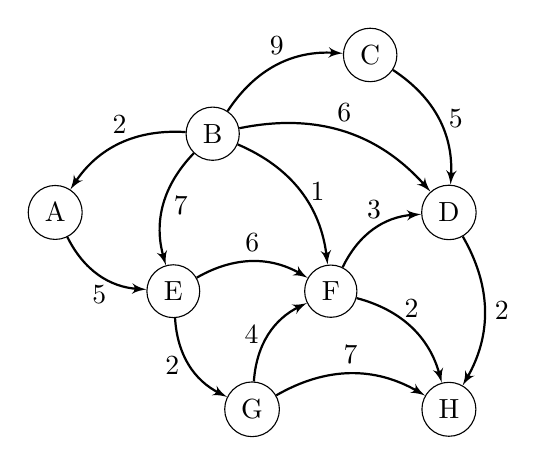
\begin{tikzpicture}
\tikzset{vertex/.style = {shape=circle,draw,minimum size=1.5em}}
\tikzset{edge/.style = {->,> = latex',thick}}
% vertices
\node[vertex] (a) at  (0,0)   {A};
\node[vertex] (b) at  (2,1)   {B};
\node[vertex] (c) at  (4,2)   {C};
\node[vertex] (d) at  (5,0)   {D};
\node[vertex] (e) at  (1.5,-1)  {E};
\node[vertex] (f) at  (3.5,-1)  {F};
\node[vertex] (g) at  (2.5,-2.5) {G};
\node[vertex] (h) at  (5,-2.5)  {H};
%edges
\draw[edge] (b) to[bend right, above] node {$2$} (a);
\draw[edge] (b) to[bend left,  above] node {$9$} (c);
\draw[edge] (b) to[bend left,  above] node {$6$} (d);
\draw[edge] (c) to[bend left,  right] node {$5$} (d);
\draw[edge] (d) to[bend left,  right] node {$2$} (h);
\draw[edge] (b) to[bend right, right] node {$7$} (e);
\draw[edge] (f) to[bend left,  above] node {$3$} (d);
\draw[edge] (e) to[bend left,  above] node {$6$} (f);
\draw[edge] (e) to[bend right,  left] node {$2$} (g);
\draw[edge] (g) to[bend left,   left] node {$4$} (f);
\draw[edge] (g) to[bend left,  above] node {$7$} (h);
\draw[edge] (a) to[bend right, below] node {$5$} (e);
\draw[edge] (f) to[bend left,  above] node {$2$} (h);
\draw[edge] (b) to[bend left,  right] node {$1$} (f);
\end{tikzpicture}
\end{center}


\subsection*{Solution}

\textbf{Source}: $B$

\textbf{Sink}: $H$

\textbf{Algorithm iterations:}

\begin{enumerate}
    \item Iteration 1:
    \begin{enumerate}
        \item $BDH$
        \item $2$
        \item Residual network:
        \begin{center}
        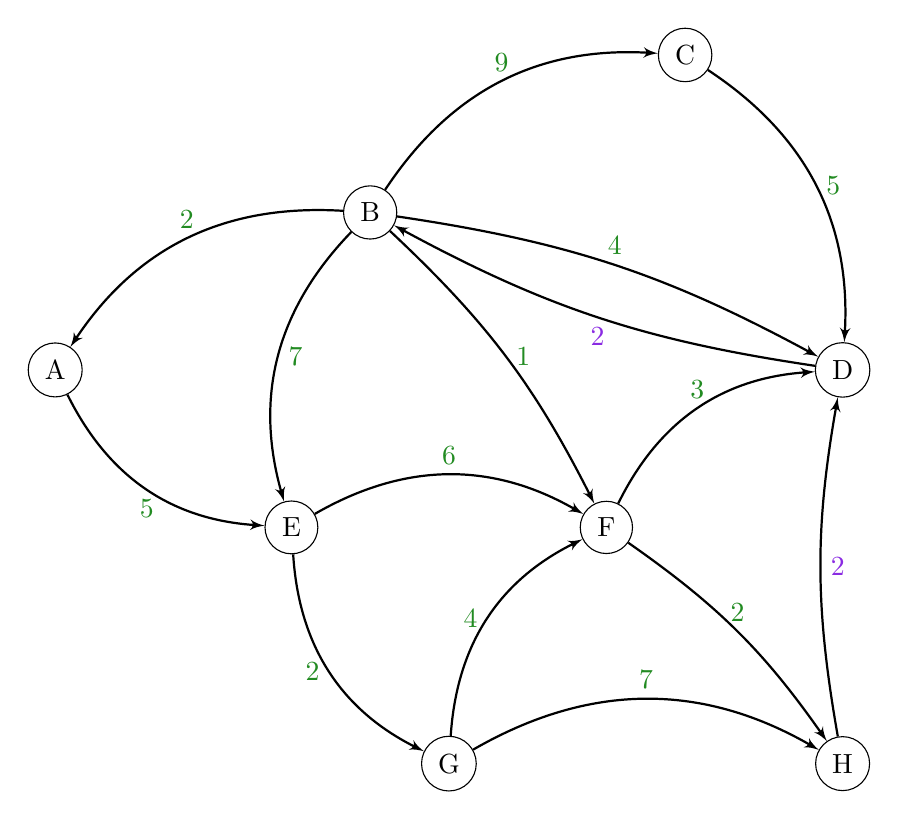
\begin{tikzpicture}
        \tikzset{vertex/.style = {shape=circle,draw,minimum size=1.5em}}
        \tikzset{edge/.style = {->,> = latex',thick}}
        % vertices
        \node[vertex] (a) at  (0,0)   {A};
        \node[vertex] (b) at  (4,2)   {B};
        \node[vertex] (c) at  (8,4)   {C};
        \node[vertex] (d) at  (10,0)   {D};
        \node[vertex] (e) at  (3,-2)  {E};
        \node[vertex] (f) at  (7,-2)  {F};
        \node[vertex] (g) at  (5,-5) {G};
        \node[vertex] (h) at  (10,-5)  {H};
        %edges
        \draw[edge] (b) to[bend right, above] node {$\textcolor{ForestGreen}{2}$} (a);
        \draw[edge] (b) to[bend left,  above] node {$\textcolor{ForestGreen}{9}$} (c);
        \draw[edge] (b) to[bend left=10,  above] node {$\textcolor{ForestGreen}{4}$} (d);
        \draw[edge] (d) to[bend left=10,  below] node {$\textcolor{BlueViolet}{2}$} (b);
        \draw[edge] (c) to[bend left,  right] node {$\textcolor{ForestGreen}{5}$} (d);
        \draw[edge] (h) to[bend left=10,  right] node {$\textcolor{BlueViolet}{2}$} (d);
        \draw[edge] (b) to[bend right, right] node {$\textcolor{ForestGreen}{7}$} (e);
        \draw[edge] (f) to[bend left,  above] node {$\textcolor{ForestGreen}{3}$} (d);
        \draw[edge] (e) to[bend left,  above] node {$\textcolor{ForestGreen}{6}$} (f);
        \draw[edge] (e) to[bend right,  left] node {$\textcolor{ForestGreen}{2}$} (g);
        \draw[edge] (g) to[bend left,   left] node {$\textcolor{ForestGreen}{4}$} (f);
        \draw[edge] (g) to[bend left,  above] node {$\textcolor{ForestGreen}{7}$} (h);
        \draw[edge] (a) to[bend right, below] node {$\textcolor{ForestGreen}{5}$} (e);
        \draw[edge] (f) to[bend left=10,  above] node {$\textcolor{ForestGreen}{2}$} (h);
        \draw[edge] (b) to[bend left=10,  right] node {$\textcolor{ForestGreen}{1}$} (f);
        \end{tikzpicture}
        \end{center}
    \end{enumerate}
    \item Iteration 2:
    \begin{enumerate}
        \item $BFH$
        \item $3$
        \item Residual network:
        \begin{center}
        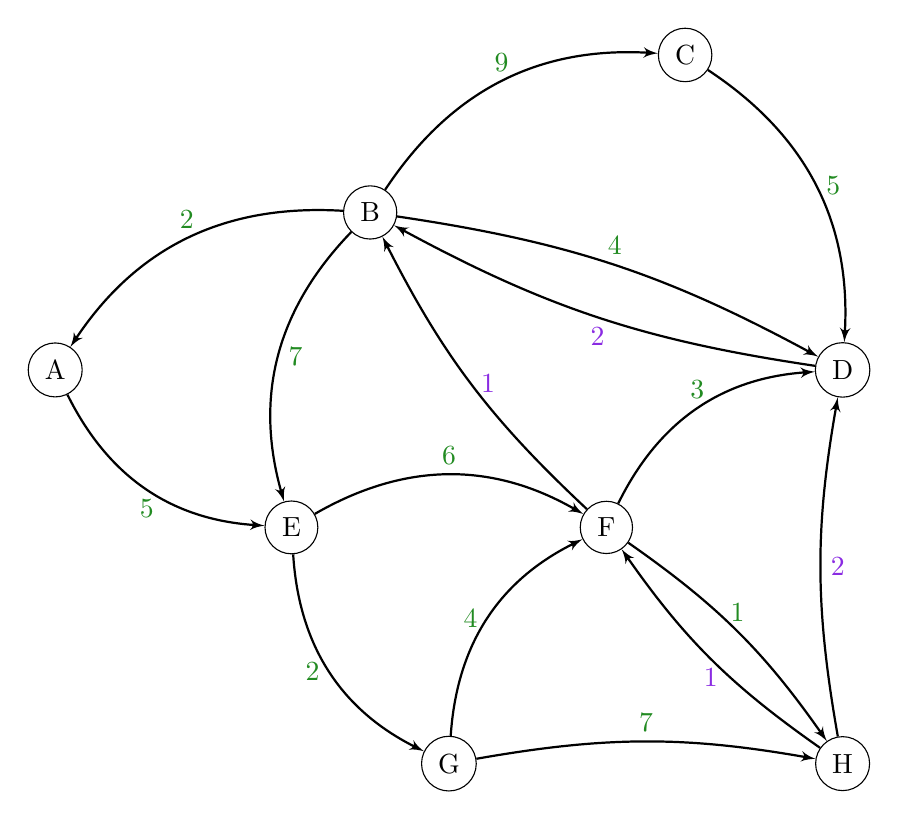
\begin{tikzpicture}
        \tikzset{vertex/.style = {shape=circle,draw,minimum size=1.5em}}
        \tikzset{edge/.style = {->,> = latex',thick}}
        % vertices
        \node[vertex] (a) at  (0,0)   {A};
        \node[vertex] (b) at  (4,2)   {B};
        \node[vertex] (c) at  (8,4)   {C};
        \node[vertex] (d) at  (10,0)   {D};
        \node[vertex] (e) at  (3,-2)  {E};
        \node[vertex] (f) at  (7,-2)  {F};
        \node[vertex] (g) at  (5,-5) {G};
        \node[vertex] (h) at  (10,-5)  {H};
        %edges
        \draw[edge] (b) to[bend right, above] node {$\textcolor{ForestGreen}{2}$} (a);
        \draw[edge] (b) to[bend left,  above] node {$\textcolor{ForestGreen}{9}$} (c);
        \draw[edge] (b) to[bend left=10,  above] node {$\textcolor{ForestGreen}{4}$} (d);
        \draw[edge] (d) to[bend left=10,  below] node {$\textcolor{BlueViolet}{2}$} (b);
        \draw[edge] (c) to[bend left,  right] node {$\textcolor{ForestGreen}{5}$} (d);
        \draw[edge] (h) to[bend left=10,  right] node {$\textcolor{BlueViolet}{2}$} (d);
        \draw[edge] (b) to[bend right, right] node {$\textcolor{ForestGreen}{7}$} (e);
        \draw[edge] (f) to[bend left,  above] node {$\textcolor{ForestGreen}{3}$} (d);
        \draw[edge] (e) to[bend left,  above] node {$\textcolor{ForestGreen}{6}$} (f);
        \draw[edge] (e) to[bend right,  left] node {$\textcolor{ForestGreen}{2}$} (g);
        \draw[edge] (g) to[bend left,   left] node {$\textcolor{ForestGreen}{4}$} (f);
        \draw[edge] (g) to[bend left=10,  above] node {$\textcolor{ForestGreen}{7}$} (h);
        \draw[edge] (a) to[bend right, below] node {$\textcolor{ForestGreen}{5}$} (e);
        \draw[edge] (f) to[bend left=10,  above] node {$\textcolor{ForestGreen}{1}$} (h);
        \draw[edge] (h) to[bend left=10,  below] node {$\textcolor{BlueViolet}{1}$} (f);
        \draw[edge] (f) to[bend left=10,  right] node {$\textcolor{BlueViolet}{1}$} (b);
        \end{tikzpicture}
        \end{center}
    \end{enumerate}
    \item Iteration 3:
    \begin{enumerate}
        \item $BEFH$
        \item $4$
        \item Residual network:
        \begin{center}
        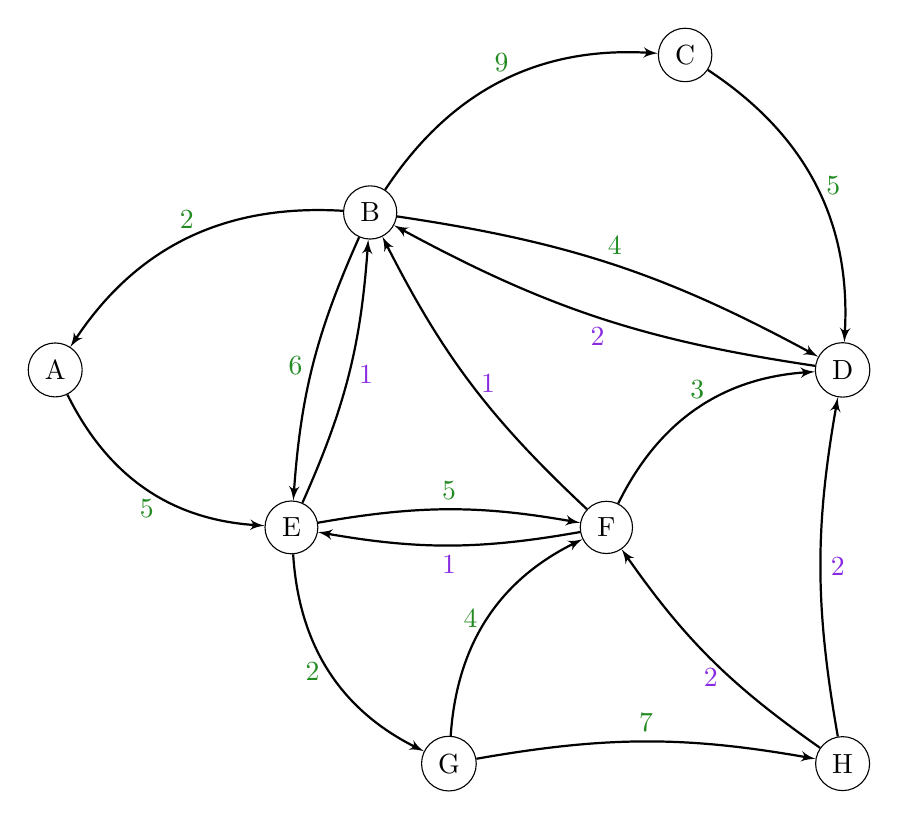
\begin{tikzpicture}
        \tikzset{vertex/.style = {shape=circle,draw,minimum size=1.5em}}
        \tikzset{edge/.style = {->,> = latex',thick}}
        % vertices
        \node[vertex] (a) at  (0,0)   {A};
        \node[vertex] (b) at  (4,2)   {B};
        \node[vertex] (c) at  (8,4)   {C};
        \node[vertex] (d) at  (10,0)   {D};
        \node[vertex] (e) at  (3,-2)  {E};
        \node[vertex] (f) at  (7,-2)  {F};
        \node[vertex] (g) at  (5,-5) {G};
        \node[vertex] (h) at  (10,-5)  {H};
        %edges
        \draw[edge] (b) to[bend right, above] node {$\textcolor{ForestGreen}{2}$} (a);
        \draw[edge] (b) to[bend left,  above] node {$\textcolor{ForestGreen}{9}$} (c);
        \draw[edge] (b) to[bend left=10,  above] node {$\textcolor{ForestGreen}{4}$} (d);
        \draw[edge] (d) to[bend left=10,  below] node {$\textcolor{BlueViolet}{2}$} (b);
        \draw[edge] (c) to[bend left,  right] node {$\textcolor{ForestGreen}{5}$} (d);
        \draw[edge] (h) to[bend left=10,  right] node {$\textcolor{BlueViolet}{2}$} (d);
        \draw[edge] (b) to[bend right=10, left] node {$\textcolor{ForestGreen}{6}$} (e);
        \draw[edge] (e) to[bend right=10, right] node {$\textcolor{BlueViolet}{1}$} (b);
        \draw[edge] (f) to[bend left,  above] node {$\textcolor{ForestGreen}{3}$} (d);
        \draw[edge] (e) to[bend left=10,  above] node {$\textcolor{ForestGreen}{5}$} (f);
        \draw[edge] (f) to[bend left=10,  below] node {$\textcolor{BlueViolet}{1}$} (e);
        \draw[edge] (e) to[bend right,  left] node {$\textcolor{ForestGreen}{2}$} (g);
        \draw[edge] (g) to[bend left,   left] node {$\textcolor{ForestGreen}{4}$} (f);
        \draw[edge] (g) to[bend left=10,  above] node {$\textcolor{ForestGreen}{7}$} (h);
        \draw[edge] (a) to[bend right, below] node {$\textcolor{ForestGreen}{5}$} (e);
        \draw[edge] (h) to[bend left=10,  below] node {$\textcolor{BlueViolet}{2}$} (f);
        \draw[edge] (f) to[bend left=10,  right] node {$\textcolor{BlueViolet}{1}$} (b);
        \end{tikzpicture}
        \end{center}
    \end{enumerate}
    \item Iteration 4:
    \begin{enumerate}
        \item $BEGH$
        \item $6$
        \item Residual network:
        \begin{center}
        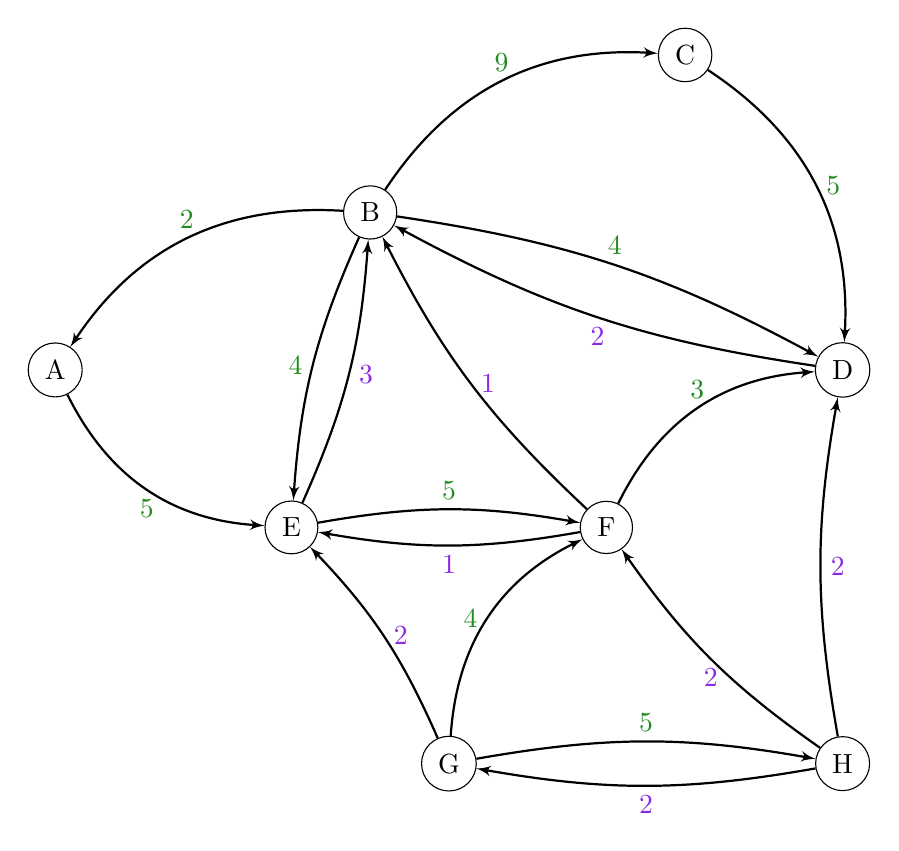
\begin{tikzpicture}
        \tikzset{vertex/.style = {shape=circle,draw,minimum size=1.5em}}
        \tikzset{edge/.style = {->,> = latex',thick}}
        % vertices
        \node[vertex] (a) at  (0,0)   {A};
        \node[vertex] (b) at  (4,2)   {B};
        \node[vertex] (c) at  (8,4)   {C};
        \node[vertex] (d) at  (10,0)   {D};
        \node[vertex] (e) at  (3,-2)  {E};
        \node[vertex] (f) at  (7,-2)  {F};
        \node[vertex] (g) at  (5,-5) {G};
        \node[vertex] (h) at  (10,-5)  {H};
        %edges
        \draw[edge] (b) to[bend right, above] node {$\textcolor{ForestGreen}{2}$} (a);
        \draw[edge] (b) to[bend left,  above] node {$\textcolor{ForestGreen}{9}$} (c);
        \draw[edge] (b) to[bend left=10,  above] node {$\textcolor{ForestGreen}{4}$} (d);
        \draw[edge] (d) to[bend left=10,  below] node {$\textcolor{BlueViolet}{2}$} (b);
        \draw[edge] (c) to[bend left,  right] node {$\textcolor{ForestGreen}{5}$} (d);
        \draw[edge] (h) to[bend left=10,  right] node {$\textcolor{BlueViolet}{2}$} (d);
        \draw[edge] (b) to[bend right=10, left] node {$\textcolor{ForestGreen}{4}$} (e);
        \draw[edge] (e) to[bend right=10, right] node {$\textcolor{BlueViolet}{3}$} (b);
        \draw[edge] (f) to[bend left,  above] node {$\textcolor{ForestGreen}{3}$} (d);
        \draw[edge] (e) to[bend left=10,  above] node {$\textcolor{ForestGreen}{5}$} (f);
        \draw[edge] (f) to[bend left=10,  below] node {$\textcolor{BlueViolet}{1}$} (e);
        \draw[edge] (g) to[bend right=10,  right] node {$\textcolor{BlueViolet}{2}$} (e);
        \draw[edge] (g) to[bend left,   left] node {$\textcolor{ForestGreen}{4}$} (f);
        \draw[edge] (g) to[bend left=10,  above] node {$\textcolor{ForestGreen}{5}$} (h);
        \draw[edge] (h) to[bend left=10,  below] node {$\textcolor{BlueViolet}{2}$} (g);
        \draw[edge] (a) to[bend right, below] node {$\textcolor{ForestGreen}{5}$} (e);
        \draw[edge] (h) to[bend left=10,  below] node {$\textcolor{BlueViolet}{2}$} (f);
        \draw[edge] (f) to[bend left=10,  right] node {$\textcolor{BlueViolet}{1}$} (b);
        \end{tikzpicture}
        \end{center}
    \end{enumerate}
\end{enumerate}

\textbf{Maximum flow value:} $6$

\textbf{Minimum cut of the network:}

\begin{center}
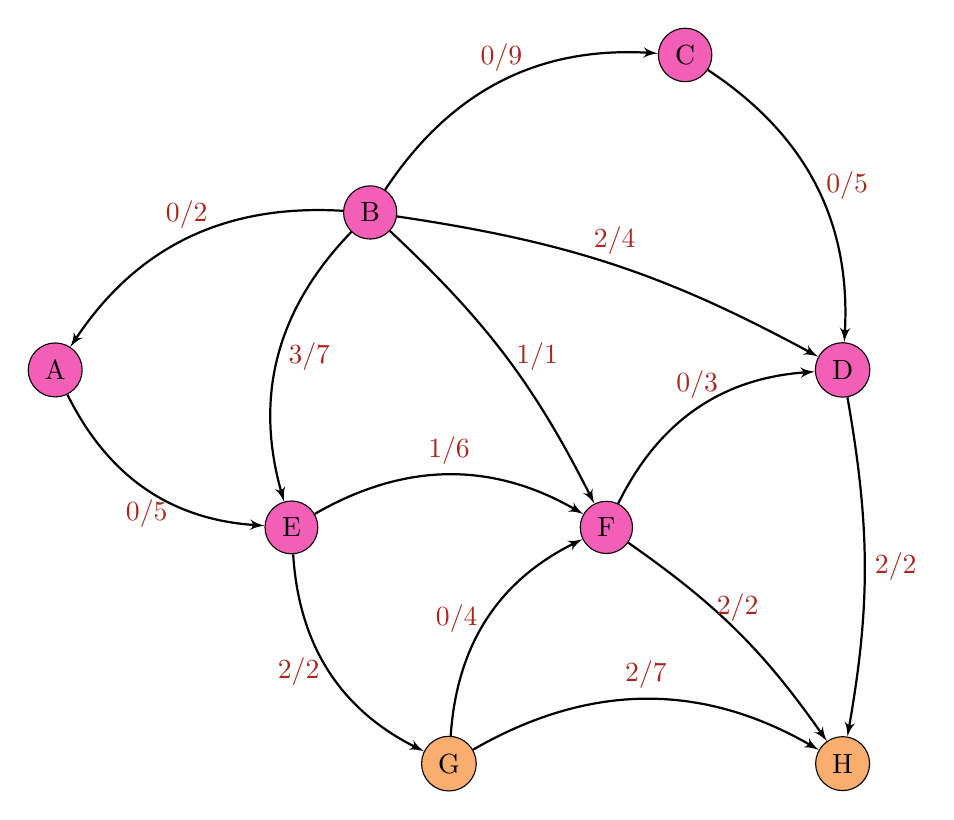
\begin{tikzpicture}
\tikzset{vertex/.style = {shape=circle,draw,minimum size=1.5em}}
\tikzset{edge/.style = {->,> = latex',thick}}
% vertices
\node[vertex, fill=CarnationPink] (a) at  (0,0)   {A};
\node[vertex, fill=CarnationPink] (b) at  (4,2)   {B};
\node[vertex, fill=CarnationPink] (c) at  (8,4)   {C};
\node[vertex, fill=CarnationPink] (d) at  (10,0)   {D};
\node[vertex, fill=CarnationPink] (e) at  (3,-2)  {E};
\node[vertex, fill=CarnationPink] (f) at  (7,-2)  {F};
\node[vertex, fill=Apricot] (g) at  (5,-5) {G};
\node[vertex, fill=Apricot] (h) at  (10,-5)  {H};
%edges
\draw[edge] (b) to[bend right, above] node {$\textcolor{Mahogany}{0/2}$} (a);
\draw[edge] (b) to[bend left,  above] node {$\textcolor{Mahogany}{0/9}$} (c);
\draw[edge] (b) to[bend left=10,  above] node {$\textcolor{Mahogany}{2/4}$} (d);
\draw[edge] (c) to[bend left,  right] node {$\textcolor{Mahogany}{0/5}$} (d);
\draw[edge] (d) to[bend left=10,  right] node {$\textcolor{Mahogany}{2/2}$} (h);
\draw[edge] (b) to[bend right, right] node {$\textcolor{Mahogany}{3/7}$} (e);
\draw[edge] (f) to[bend left,  above] node {$\textcolor{Mahogany}{0/3}$} (d);
\draw[edge] (e) to[bend left,  above] node {$\textcolor{Mahogany}{1/6}$} (f);
\draw[edge] (e) to[bend right,  left] node {$\textcolor{Mahogany}{2/2}$} (g);
\draw[edge] (g) to[bend left,   left] node {$\textcolor{Mahogany}{0/4}$} (f);
\draw[edge] (g) to[bend left,  above] node {$\textcolor{Mahogany}{2/7}$} (h);
\draw[edge] (a) to[bend right, below] node {$\textcolor{Mahogany}{0/5}$} (e);
\draw[edge] (f) to[bend left=10,  above] node {$\textcolor{Mahogany}{2/2}$} (h);
\draw[edge] (b) to[bend left=10,  right] node {$\textcolor{Mahogany}{1/1}$} (f);
\end{tikzpicture}
\end{center}

The flow across the cut is equal to $2 + 2 + 2 - 0 = 6$, therefore, the found value is correct.

\begin{thebibliography}{9}
\bibitem{Cormen}
  T. H. Cormen, C. E. Leiserson, R. L. Rivest and C. Stein.
  \textit{Introduction to Algorithms, Fourth Edition.}
  The MIT Press
  2022.
\end{thebibliography}

\end{document}
